\chapter{Conception} \label{chap:conception}

\section*{}

In this chapter is clarified and presented the scope of the project and the exploration of the solution.

\section{Assessment Process} \label{sec:Approach}

The Electronic assessment process is represented in Figure \ref{fig:assessmentprocess}.
The process starts with a selection of the projects needed to evaluate and process areas to evaluate; then for each evaluation, we have two ongoing tasks. These ongoing tasks are the Survey based electronic assessment and the Rule based assessment.

The Survey based electronic assessment is a manual process where the user needs to answer the questions that are provided. The Rule based electronic assessment is fully automatic using the rules conceived in this thesis.

Both these assessments receive Project data to generate the results that can be seen afterwards. In this model is present too the manual adjustment, a part that can be useful if in some case a certain part is not evaluated correctly or the assessment result is by consented opinion of the team accepted or rejected. And for last is shown the final results. 

The details of rule based and survey based assessment are provided in section \ref{sec:mapping} and \ref{sec:question}.

In order to get a full overview of the Scraim, an assessment of the tool was performed. That assessment provides the current state of the tool and possible gaps to workaround.
After analyzing the gaps a map can be done, that map was done between CMMI for development practices and the tool.

\begin{landscape}
	\begin{figure}[h]
		\begin{center}
			\leavevmode
			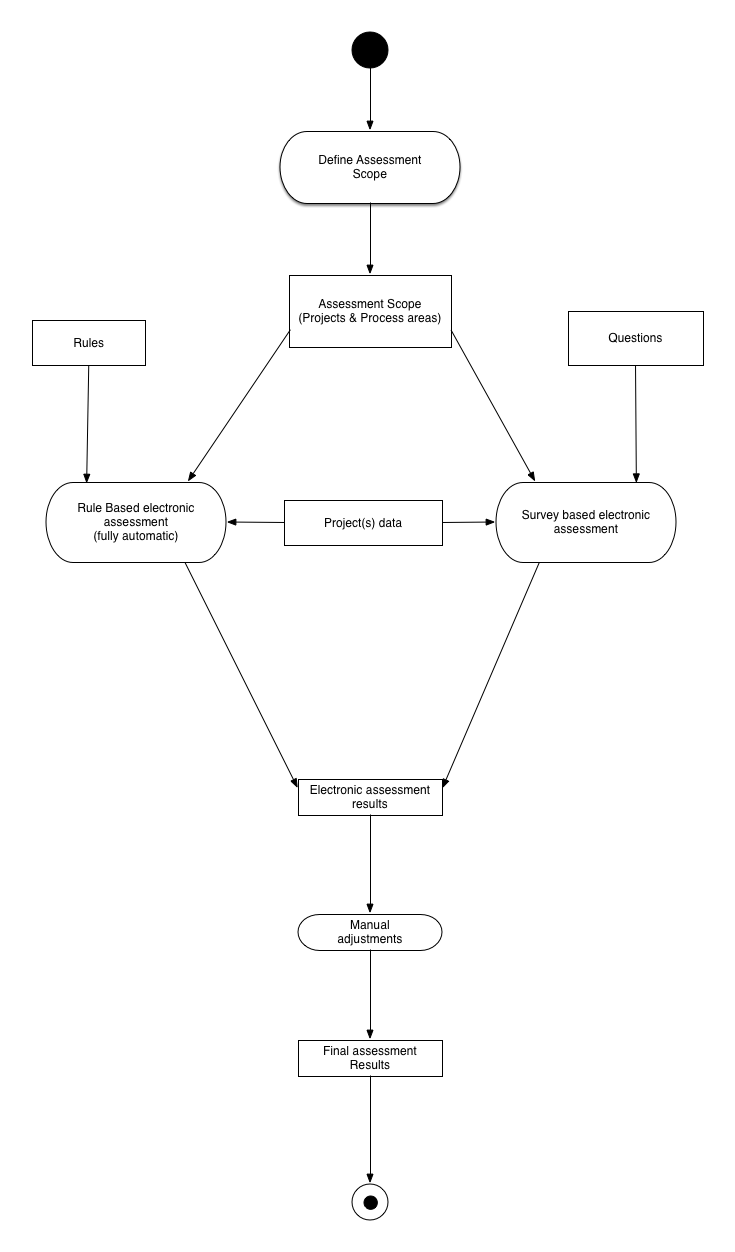
\includegraphics[width=1.6\textwidth]{assessmentprocess}
			\caption{Assessment Process Workflow}
			\label{fig:assessmentprocess}
		\end{center}
	\end{figure}
\end{landscape}

\section{Pre-Assessment of Scraim Support} \label{sec:preassessment}

In a primary phase as mentioned before, an assessment of the tool was performed. The actual purpose of this assessment was to check if it was possible and currently viable to match Scraim and its functionalities with the third maturity level of CMMI for Development.

Maturity levels comprise a set of process areas, measured by the respective goals of those areas and their practices. So if Scraim could be mapped to a more extensive number of practices and goals, a higher level of maturity could be covered.

The assessment was done with Appraisal Assistant, a tool currently used to assist and help appraisals in the field(see section \ref{chap:chap3}). This tool allows to show the results in a matrix providing a full overview of the current state and the coverage of Scraim in relation to the maturity level 3 of CMMI for Development.


\begin{figure}[h]
	\begin{center}
		\leavevmode
		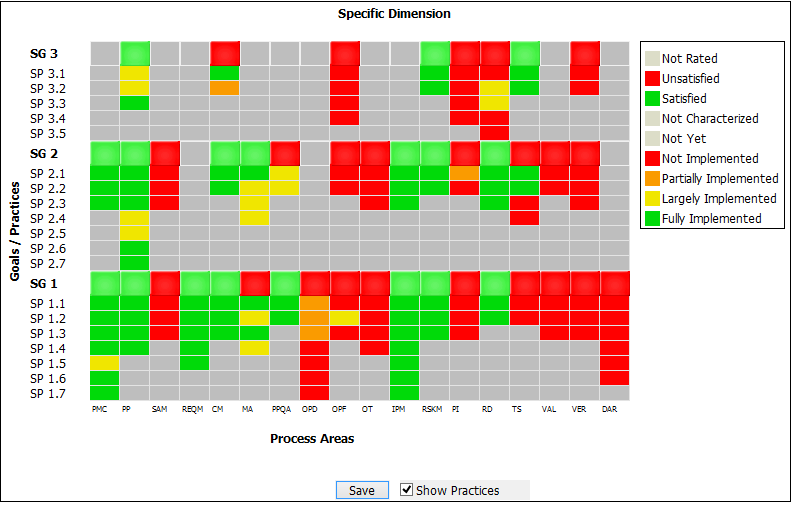
\includegraphics[width=0.8\textwidth]{Level_3}
		\caption{Scraim Assessment to CMMI for Development Level 3}
		\label{fig:level3}
	\end{center}
\end{figure}

In Figure \ref{fig:level3} we can see that despite the fact that Scraim covers many practices, the maturity level three is still too far from being achieved successfully.

For example some areas like Verification (VER) and Decision Analysis and Resolution (DAR), are not currently supported by SCRAIM, so it will be impossible to automatically assess the fulfillment of their respective goals and practices by SCRAIM users.

The maturity level 2 is chosen to make a more precise and accurate coverage of CMMI practices and be able to map.

In Figure \ref{fig:level2} we can see that the map for the second level of maturity is more accurate, more trustful and can be more covered automatically.
	
\begin{figure}[h]
	\begin{center}
		\leavevmode
		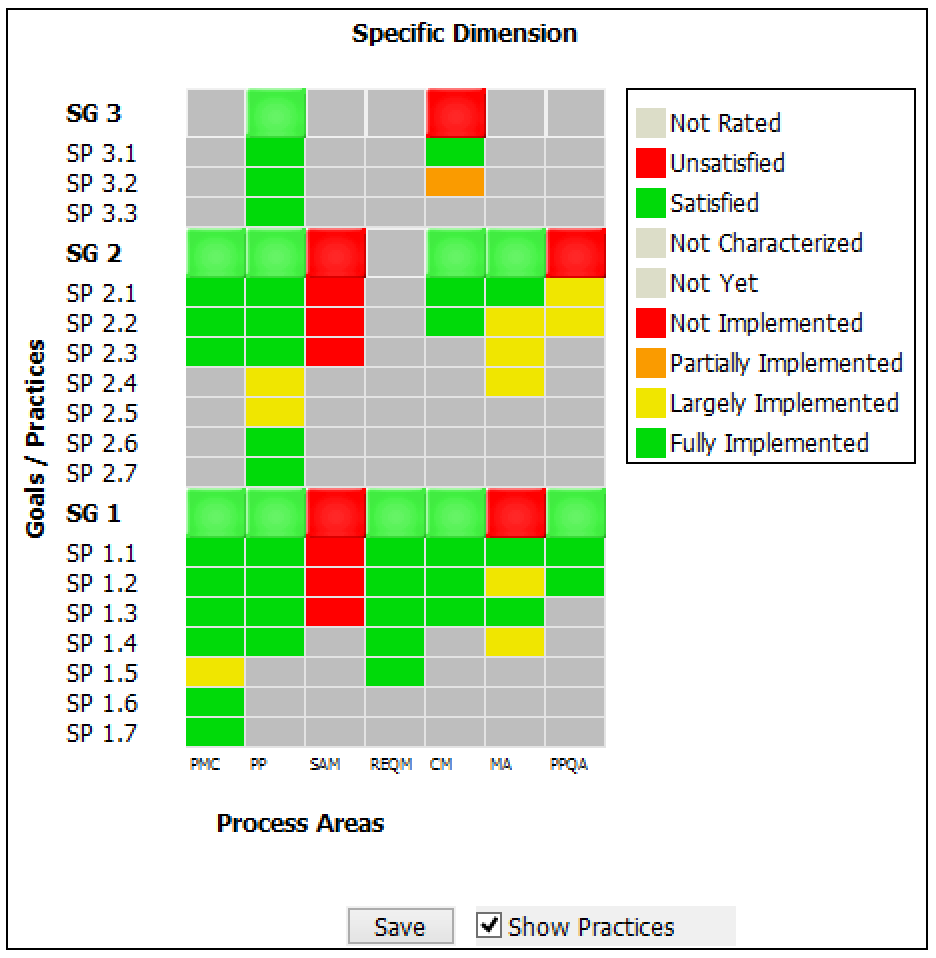
\includegraphics[width=0.7\textwidth]{Level_2}
		\caption{Scraim Assessment to CMMI for Development Level 2}
		\label{fig:level2}
	\end{center}
\end{figure}

The previous decision of making this set of tools to Scraim focusing in the level two is supported by these two assessments to the tool.



\section{Electronic Assessment Rules} \label{sec:mapping}
In order to get rules it was needed to do a CMMI-SCRAIM map. 
This map is where it has been evaluated the data model items and the level of support available on SCRAIM and match them to CMMI best practices.

Taking as reference the previous assessments of the tool, this map was possible with the creation of a new scale to show the results of the assessment and be possible the map corresponding the information.

One appraisal consists in classifying each practice in one of four states: Fully Implemented, Largely Implemented, Partially implemented and Not implemented.

\begin{figure}[h]
	\begin{center}
		\leavevmode
		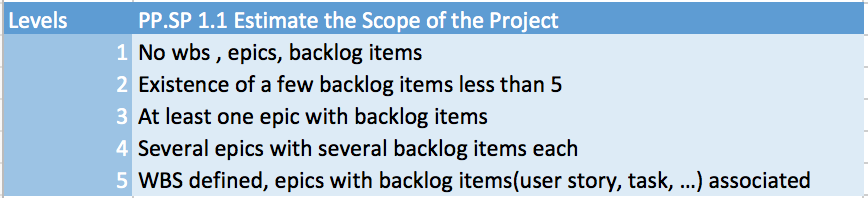
\includegraphics[width=0.6\textwidth]{mapping_5levels}
		\caption{Project Planning SP1.1 Map to 5 levels}
		\label{fig:mapping_5levels}
	\end{center}
\end{figure}

In the first attempt, was tried to match those levels with 5 levels, corresponding to different evaluation levels in Scraim. In the Figure \ref{fig:mapping_5levels} is possible to see the map between CMMI for Development and Scraim. In this example is analyzed the criteria from the practice 1.1 from the Project Planning area, which says, "Establish a top-level work breakdown structure (WBS) to estimate the scope of the project." and can be mapped into Scraim into this 5 levels. The first Level would be where there is none WBS item or backlog item, and the max level where all WBS are fully defined and epics with backlog items associated. 

\begin{figure}[h]
	\begin{center}
		\leavevmode
		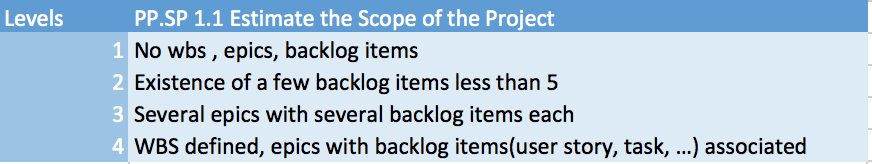
\includegraphics[width=0.6\textwidth]{mapping_4levels}
		\caption{Project Planning SP1.1 Map to 4 levels}
		\label{fig:mapping_4levels}
	\end{center}
\end{figure}

After some mapping this scale was confusing and far from real so the best way was to map and try match the four levels of SCAMPI with four levels of Scraim assessment.

This new scale is more accurate and closer to a real assessment. In the Figure \ref{fig:mapping_4levels} is observable that the mid levels are more easily distinguished and more differentiable from the others. 

\section{Electronic Assessment Questions} \label{sec:question}

Regarding the mapping, it was discovered  that some practices can not be automatically evaluated so another way of providing some results needs to be found.

The founded way is make an survey of pre-established questions. Those questions derived from CMMI assessment checklists and tools and ITMARK Appraisal tool will guarantee closer results and a more wider assessment.

\section{Recommendations for extending the Scraim Support}

Some of the gaps found can be solved with the integration of some Plugins, some frameworks and some rules of usage.

Rules, frameworks and Plugins:
\begin{itemize}
	\item Plugin for wiki templates
	
	This plugin allows to choose a wiki template when is added a new page. It is possible see a preview of the template before choose it.
	This plugin will allow to resolve and input information directly in Scraim, without the use of other programs to generate those documents.
	
	\item Plugin for Document Management System Features
	
	Allows to manage documents submitted on Scraim, document approval workflow to be configurable and maintain a version control of this documents.
	
	\item Certain names for submitted documents
	
	For example the Project plan must be submitted with a certain name to the Scraim files, to be automatic evaluated or it will not be considered.
	
\end{itemize}